\usetikzlibrary{positioning,fit,matrix}
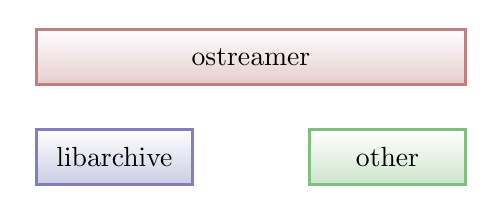
\begin{tikzpicture}[
  redblock/.style={
    rectangle,
    very thick,
    draw=red!50!black!50,
    top color=white,
    bottom color=red!50!black!20,
    inner sep=0em,
    minimum width=17mm,
    minimum height=2em
  },
 blueblock/.style={
    rectangle,
    very thick,
    draw=blue!50!black!50,
    top color=white,
    bottom color=blue!50!black!20,
    inner sep=0em,
    minimum width=17mm,
    minimum height=2em
  },
 greenblock/.style={
    rectangle,
    very thick,
    draw=green!50!black!50,
    top color=white,
    bottom color=green!50!black!20,
    inner sep=0em,
    minimum width=17mm,
    minimum height=2em
  }]
  \matrix (table) [
    %draw
    matrix of nodes,
    nodes in empty cells,
    row sep=4mm,
    column sep = 15mm,
   nodes={text centered}] {
   & & & \\
   & & & \\
   & & & \\
   };
  \node[fit=(table-1-1)(table-1-4),redblock,label={center:ostreamer}]{};
  \node[fit=(table-3-1)(table-3-2),blueblock,label={center:libarchive}] {};
  \node[fit=(table-3-3)(table-3-4),greenblock,label={center:other}] {};
\end{tikzpicture}
% http://tex.stackexchange.com/questions/94343/matrix-of-nodes-over-multiple-columns-in-tikz